\documentclass[a4paper,12pt]{article}
\usepackage{natbib,setspace,amsmath,graphicx,float,booktabs}
\usepackage[skip=0.5\baselineskip]{caption}
\usepackage{adjustbox}
\onehalfspacing
\newcommand{\bs}[1]{\boldsymbol{#1}}
\setlength\parindent{0pt}

\begin{document}

\begin{titlepage}
\noindent
\includegraphics[width=5cm]{uzh_logo_e_pos.pdf}
\noindent{\bf Department of Economics}
\noindent\rule{\textwidth}{0.4pt}
\vspace{1cm}
  \begin{center}
		{\LARGE Using AS-AD framework and VAR model to [...] Interwar US} \\
		{\Large Quantitative Economic History - Applications\\Spring Term 2021}
  \end{center}
\vfill

{\flushleft
Hubert Mrugala \\
Banking and Finance\\
hubert.mrugala@uzh.ch\\
19764265}  

\end{titlepage}

\pagebreak
\pagebreak

\section{Introduction}

Aaa.
\newpage

\section{Data}

The dataset consists of 252 monthly observations of American Industrial Production (IP) and Consumer Index Prices (CPI) from January 1919 to December 1939. The data can be split into two periods, i.e. pre-great depression and post great depression. The first one I define as the time between the beginning of the data sample, January 1919, to the upper-turning point in May 1929, the second one follows from that point to the end of the time-series. After the war there is a sharp increase in the price level index from 57 in the beginning of 1919 to 70 in mid 1920s. Then, prices deflate to about 59 (Depression of 1920-1921) and stay around that level until February 1931, when CPI falls below 55. Not surprisingly years 1931-33 are considered to be the most severe time of the Great Depression as in this period prices were declining each month until reaching the lowest point of 43.7 in April 1933.

\begin{table}
\label{table:1}
\caption{Basic Statistics}
\centering
\input{../output/tables/stats.txt}
\end{table}

Pre-Great Depression Industrial Production, except the time of 1920-21 depression, was growing steadily. At the peak, IP was about 40 and it took almost 7 years of depression and recovery to come back to that level. At the end of the inter-war period we can also see a very sudden collapse of IP. It is the Recession of 1937-38 - third-worst recession of the twentieth century. CITE

\begin{table}
\label{table:2}
\caption{Yearly data}
\begin{adjustbox}{max width=1.1\textwidth,center}
\centering
\input{../output/tables/yearly_data.txt}
\end{adjustbox}
\end{table}



\begin{figure}[H]
    \centering
\caption{Industrial Production}
    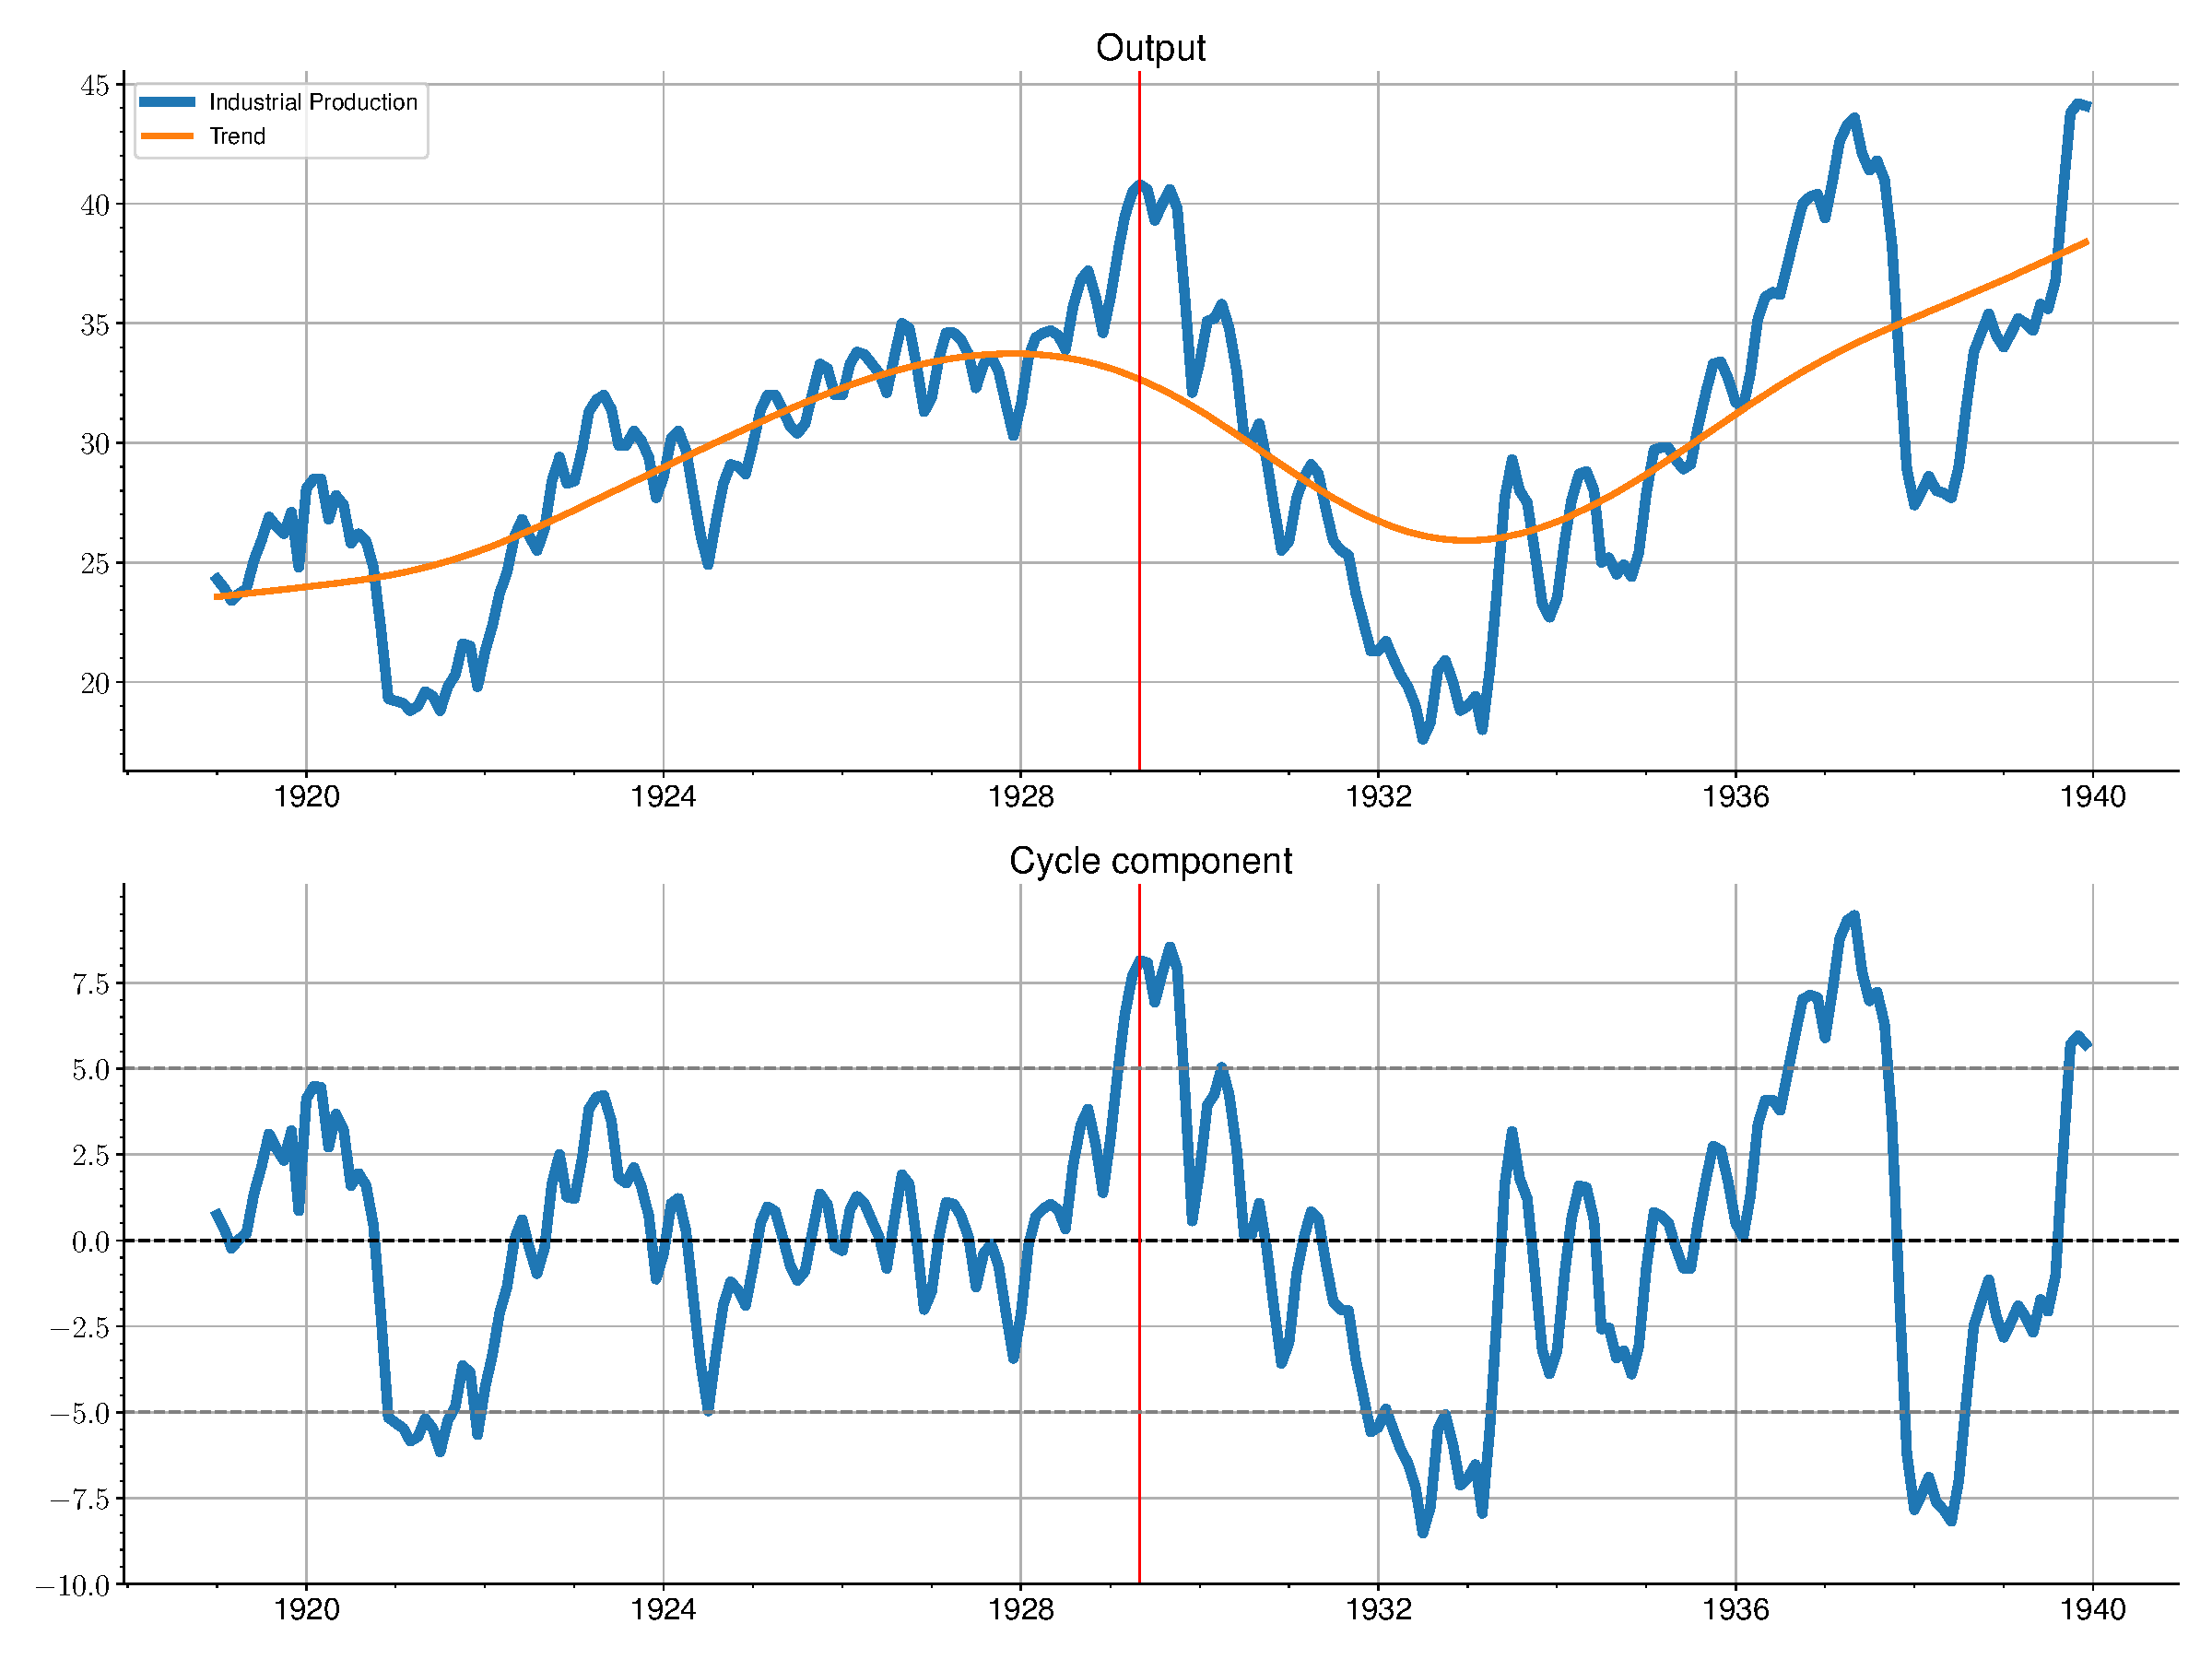
\includegraphics[width=\textwidth]{../output/figures/ts_IP.pdf} 
\end{figure}
\newpage

\begin{figure}[H]
    \centering
\caption{Consumenr Price Index}
    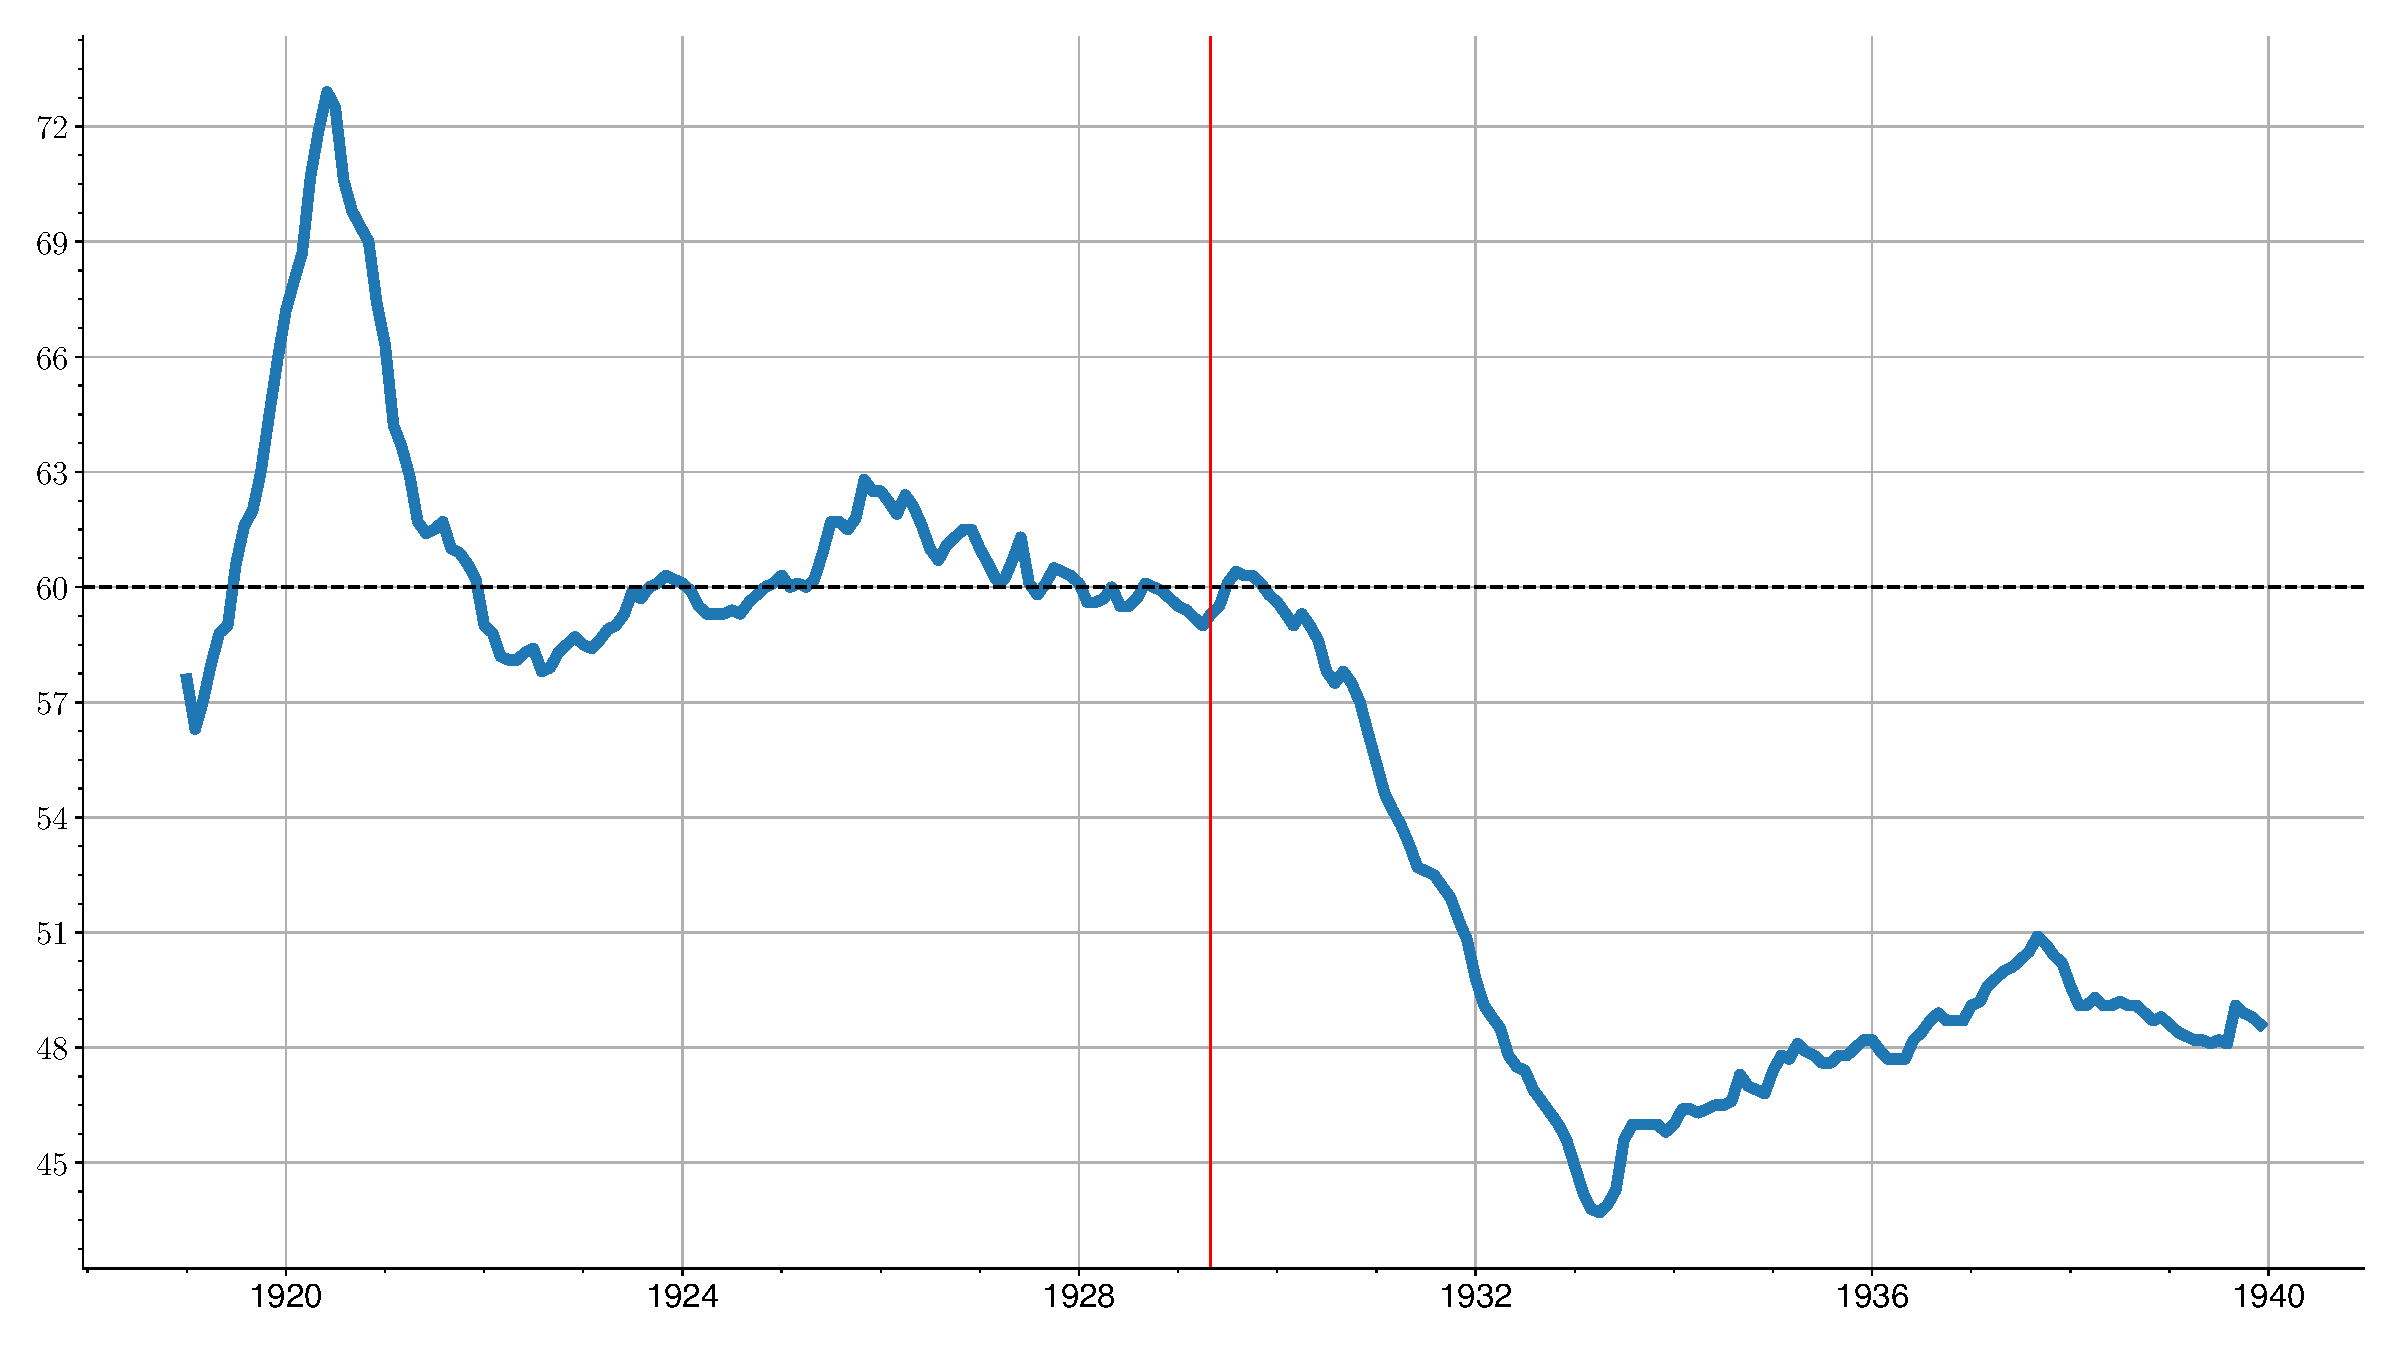
\includegraphics[width=\textwidth]{../output/figures/ts_CPI.pdf} 
\end{figure}

\section{Method}
\subsection{Vector Autoregressive Model}

To analyze relationship between two endogenous time-series, price level \(\bf M\) and output \(\bf Y\), a vector autoregression (VAR) model is used.

\begin{equation}
		{\mathbf{y_{t}=c+A_{1}y_{{t-1}}+A_{2}y_{{t-2}}+\cdots +A_{p}y_{{t-p}}+e_{t}}}
\end{equation}

In the formula above \(\bf c\) is a constant, \(\bf A_i\) are coefficient matrices and \(\bf u_i\) are error terms. When analyzing monetary transmission mechanism, VAR can be also expressed in the following form (Favero).

\begin{equation}
\begin{split}
		\mathbf{G}\left(\begin{array}{c}
		\mathbf{Y}_{t} \\
		\mathbf{M}_{t}
		\end{array}\right)=\mathbf{K}(L)\left(\begin{array}{c}
		\mathbf{Y}_{t-1} \\
		\mathbf{M}_{t-1}
		\end{array}\right)+\mathbf{F}\left(\begin{array}{c}
		\epsilon_{\mathbf{Y}, \mathbf{t}} \\
		\epsilon_{\mathbf{M}, \mathrm{t}}
		\end{array}\right)
\end{split}
\end{equation}

In the structural model above matrix \(\bf G\) represents contemporaneous relations among the variables and \(\bf K(L)\) is the matrix of finite-order lag polynomial. The model is not directly observable, however, a reduced form can be estimated.

\begin{equation}
\begin{split}
		\left(\begin{array}{c}
		\mathbf{Y}_{t} \\
		\mathbf{M}_{t}
		\end{array}\right)=\mathbf{G}^{-1} \mathbf{K}(L)\left(\begin{array}{c}
		\mathbf{Y}_{t-1} \\
		\mathbf{M}_{t-1}
		\end{array}\right)+\mathbf{G}^{-1} \mathbf{F}\left(\begin{array}{c}
		\epsilon_{\mathbf{Y}, \mathbf{t}} \\
		\epsilon_{\mathbf{M}, \mathrm{t}}
		\end{array}\right)
\end{split}
\end{equation}

In this paper, vector autoregression is used to obtain impulse responses and forecast error decompositions in the AS-AD framework. To do this, I use Blanchard-Quach decomposition where we assume that aggregate demand shocks has no long-run effect on real output. The assumption helps to solve the identification problem by imposing restictions on the impact matrix \(\bf S = G^{-1}-F\)

\begin{equation}
		\mathbf{u}_{\mathbf{t}}=\mathbf{S} \epsilon_{\mathbf{t}}
\end{equation}

To find S first lets start with the moving average representations of reduced form VAR equation 1 and the structural model eq2.

\begin{equation}
\begin{split}
		\mathbf{y}_{\mathbf{t}} &=\mathbf{B}(\mathbf{L}) \mathbf{u}_{\mathbf{t}}, \\
		\mathbf{y}_{\mathbf{t}} &=\mathbf{C}(\mathbf{L}) \epsilon_{\mathbf{t}}
\end{split}
\end{equation}

After substituting for u t and simplifying

\begin{equation}
		\mathbf{B}(L) \mathbf{S}=\mathbf{C}(L)
\end{equation}

The long-run coefficient matrix is \(\bf C(1) = B(1)S\), and so to get \(\bf S\), long-run \(\bf C(1)\) is needed. Postmultiplying C(1) with its transpose gives

\begin{equation}
		\mathbf{B}(1) \mathbf{S S}^{\prime} \mathbf{B}(1)^{\prime}=\mathbf{C}(1) \mathbf{S}^{-1} \mathbf{S} \mathbf{S}^{\prime}\left(\mathbf{S}^{\prime}\right)^{-1} \mathbf{C}(1)^{\prime}=\mathbf{C}(1) \mathbf{C}(1)^{\prime}.
\end{equation}

Cholesky decomposition of the expression above produces the restricted long-run coefficient matrix \(\bf C(1)\), that allows to calculate matrix \(\bf S\).

\subsection{Impulse Responses}

Impact matix S connects structural shocks e t to the reduced form residuals u t

\begin{equation}
		\mathbf{u}_{\mathbf{t}}=\mathbf{S} \epsilon_{\mathbf{t}}
\end{equation}

To find S first lets start with the moving average representations of reduced form VAR equation 1 and the structural model eq2.

\begin{equation}
\begin{split}
		\mathbf{y}_{\mathbf{t}} &=\mathbf{B}(\mathbf{L}) \mathbf{u}_{\mathbf{t}}, \\
		\mathbf{y}_{\mathbf{t}} &=\mathbf{C}(\mathbf{L}) \epsilon_{\mathbf{t}}
\end{split}
\end{equation}

After substituting for u t and simplifying

\begin{equation}
		\mathbf{B}(L) \mathbf{S}=\mathbf{C}(L)
\end{equation}

The long-run coefficient matrix is \(\bf C(1) = B(1)S\), and so to get \(\bf S\), long-run \(\bf C(1)\) is needed. Postmultiplying C(1) with its transpose gives

\begin{equation}
		\mathbf{B}(1) \mathbf{S S}^{\prime} \mathbf{B}(1)^{\prime}=\mathbf{C}(1) \mathbf{S}^{-1} \mathbf{S} \mathbf{S}^{\prime}\left(\mathbf{S}^{\prime}\right)^{-1} \mathbf{C}(1)^{\prime}=\mathbf{C}(1) \mathbf{C}(1)^{\prime}.
\end{equation}

Cholesky decomposition of the expression above produces the restricted long-run coefficient matrix \(\bf C(1)\), that allows to calculate matrix \(\bf S\).

\subsection{Forecast Error Variance Decomposition}

Forecast error variances for two variables \((k=1,2)\) can be expressed as

\begin{equation}
		\mathrm{E}\left[\left(y_{k, t+1}-\hat{y}_{k, t+1}\right)^{2}\right]=\mathbf{e}_{k} \mathbf{\Sigma} \mathbf{e}_{k}^{\prime}=\mathbf{e}_{k} \mathbf{S S}^{\prime} \mathbf{e}_{k}^{\prime}=\mathbf{e}_{k} \mathbf{C}_{0} \mathbf{C}_{0}^{\prime} \mathbf{e}_{k}^{\prime}.
\end{equation}

Then contribution of the the shock \(l\) to the forecast error variances of variable \(k\) at time \(h\) can be, generally, written in a for of the following three dimentional array

\begin{equation}
		\theta_{h, k l}=\frac{\sum_{j=0}^{h-1}\left(\mathbf{e}_{k} \mathbf{C}_{j} \mathbf{e}_{l}^{\prime}\right)^{2}}{\sum_{j=0}^{h-1} \mathbf{e}_{k} \mathbf{C}_{j} \mathbf{C}_{j}^{\prime} \mathbf{e}_{k}^{\prime}}
\end{equation}

\newpage

\section{Results}

\begin{table}
\label{table:3}
\caption{Restricted Long-run Responses}
\centering
\input{../output/tables/C1.txt}
\end{table}

\begin{itemize}
\item Price index:
\begin{itemize}
\item 1700-1823: \citet{schumpeter38}, in \citet[p. 468-469]{mitchelldeane71}
\item 1823-1913: \citet[p. 863-864]{mitchelle2003}
\end{itemize}

\item Industrial production: \citet[p. 725-727]{craftsharley92}

\end{itemize}

\begin{figure}[H]
    \centering
\caption{Impulse Responses}
    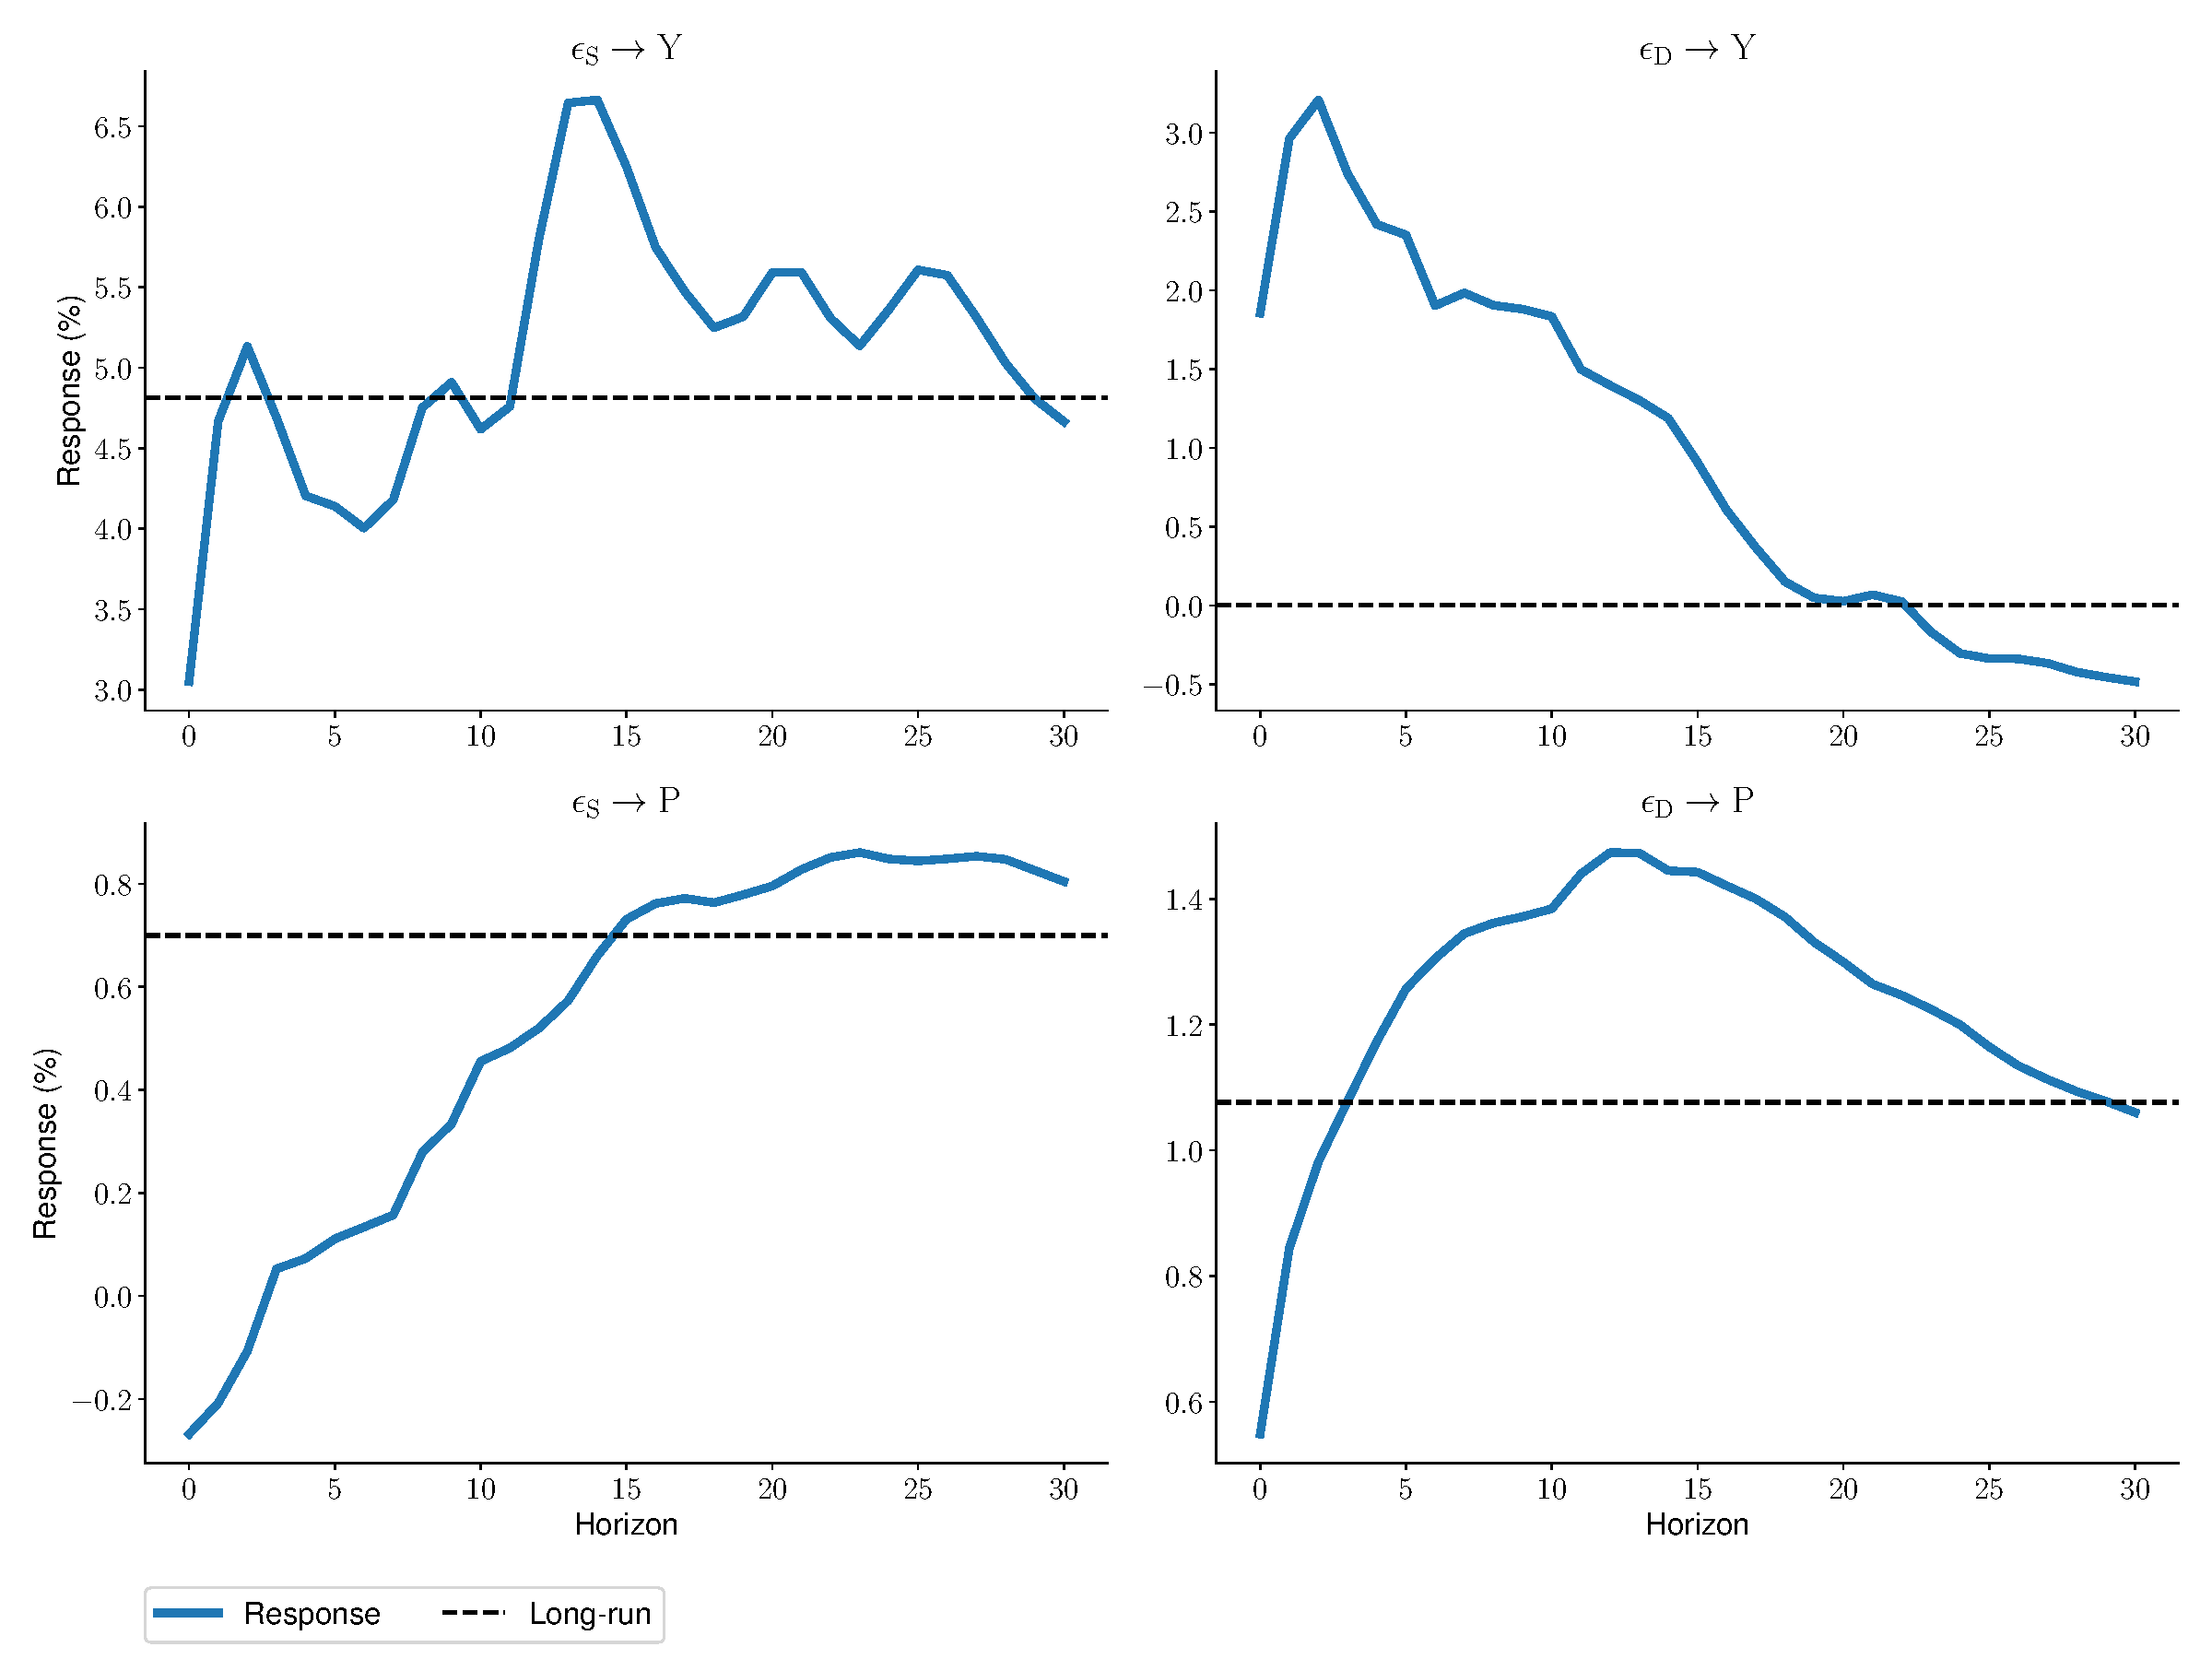
\includegraphics[width=\textwidth]{../output/figures/IR.pdf} 
\end{figure}

To be discussed.

\pagebreak

\bibliography{sqwg}
\bibliographystyle{eeh}

\end{document}
